\documentclass[journal,12pt,onecolumn]{IEEEtran}
\usepackage{cite}
\usepackage{graphicx}
\usepackage{amsmath,amssymb,amsfonts,amsthm}
\usepackage{algorithmic}
\usepackage{graphicx}
\usepackage{textcomp}
\usepackage{xcolor}
\usepackage{txfonts}
\usepackage{listings}
\usepackage{enumitem}
\usepackage{mathtools}
\usepackage{gensymb}
\usepackage{comment}
\usepackage[breaklinks=true]{hyperref}
\usepackage{tkz-euclide} 
\usepackage{listings}
\usepackage{gvv}                                        
%\def\inputGnumericTable{}                                 
\usepackage[latin1]{inputenc} 
\usetikzlibrary{arrows.meta, positioning}
\usepackage{xparse}
\usepackage{color}                                            
\usepackage{array}                                            
\usepackage{longtable}                                       
\usepackage{calc}                                             
\usepackage{multirow}
\usepackage{multicol}
\usepackage{hhline}                                           
\usepackage{ifthen}                                           
\usepackage{lscape}
\usepackage{tabularx}
\usepackage{array}
\usepackage{float}
\newtheorem{theorem}{Theorem}[section]
\newtheorem{problem}{Problem}
\newtheorem{proposition}{Proposition}[section]
\newtheorem{lemma}{Lemma}[section]
\newtheorem{corollary}[theorem]{Corollary}
\newtheorem{example}{Example}[section]
\newtheorem{definition}[problem]{Definition}
\newcommand{\BEQA}{\begin{eqnarray}}
\newcommand{\EEQA}{\end{eqnarray}}
\usepackage{float}
%\newcommand{\define}{\stackrel{\triangle}{=}}
\theoremstyle{remark}
\usepackage{circuitikz}
\usepackage{tikz}
% Marks the beginning of the document
\begin{document}
\title{2025-XH-'1-65'}
\author{EE25BTECH11020 - Darsh Pankaj Gajare}
\maketitle
\begin{enumerate}

\item If '$\rightarrow $' denotes increasing order of intensity, then the meaning of the words $\brak{simmer \rightarrow  seethe \rightarrow  smolder}$ is analogous to $\sbrak{break \rightarrow  raze \rightarrow  \rule{2cm}{0.4pt} }$. Which one of the given options is appropriate to fill the blank? 
\hfill $\brak{GATE\ EE\ 2025}$
    \begin{enumerate}
    \begin{multicols}{4}
  \item obfuscate    
  \item obliterate 
 \item fracture
  \item fissure 
  \end{multicols}
  \end{enumerate}
   \item In a locality, the houses are numbered in the following way:
The house-numbers on one side of a road are consecutive odd integers starting from 301, while the house-numbers on the other side of the road are consecutive even numbers starting from 302. The total number of houses is the same on both sides of the road.
If the difference of the sum of the house-numbers between the two sides of the road is 27, then the number of houses on each side of the road is: 
   \hfill $\brak{GATE\ EE\ 2025}$
       \begin{enumerate}
\begin{multicols}{4}
\item $27$   
  \item $52$
  \item $54$
  \item $26$ 
  \end{multicols}
  \end{enumerate}
   \item For positive integers $ p $ and $ q $, with $ \frac{p}{q} \neq 1 $, 
$\left( \frac{p}{q} \right)^q = p^{\left( \frac{p}{q} - 1 \right)},$
Then,
\hfill $\brak{GATE\ EE\ 2025}$
    \begin{enumerate}
    \begin{multicols}{4}
  \item$ q^p = p^q$  
 \item $q^p = p^{2q}$
  \item $ \sqrt{q} = \sqrt{p} $
  \item $ \sqrt[p]{q} = \frac{q}{\sqrt{p}} $    
  \end{multicols}
  \end{enumerate}
\item  Which one of the given options is a possible value of $ X $ in the following sequence?
$3,\ 7,\ 15,\ X,\ 63,\ 127,\ 255$
\hfill $\brak{GATE\ EE\ 2025}$
    \begin{enumerate}
\begin{multicols}{4}
   \item $35$   
  \item $40$
  \item $45$
  \item $31$\end{multicols}
    \end{enumerate}
\item  On a given day, how many times will the second-hand and the minute-hand of a clock cross each other during the clock time $12:05:00$ hours to $12:55:00$ hours?\\
\hfill $\brak{GATE\ EE\ 2025}$
    \begin{enumerate}
    \begin{multicols}{4}
  \item $51$ 
  \item $49$  
  \item $50$  
  \item $55$  \end{multicols}
    \end{enumerate}
\item In the given text, the blanks are numbered $\brak{i}- \brak{iv}$. Select the best match for all the blanks. From the ancient Athenian arena to the modern Olympic stadiums, athletics \underline{\brak{i}} the potential for a spectacle. The crowd \underline{\brak{ii}} with bated breath as the Olympian artist twists his body, stretching the javelin behind him. Twelve strides in, he begins to cross-step. Six cross-steps \underline{\brak{iii}} in an abrupt stop on his left foot. As his body \underline{\brak{iv}} like a door turning on a hinge, the javelin is launched skyward at a precise angle. 
\hfill $\brak{GATE\ EE\ 2025}$
    \begin{enumerate}
  \item \brak{i} hold \quad \brak{ii} waits \quad \brak{iii} culminates \quad \brak{iv} pivot  \item \brak{i} holds \quad \brak{ii} wait \quad \brak{iii} culminates \quad \brak{iv} pivot 
 \item \brak{i} hold \quad \brak{ii} wait \quad \brak{iii} culminate \quad \brak{iv} pivots  
  \item \brak{i} holds \quad \brak{ii} waits \quad \brak{iii} culminate \quad \brak{iv} pivots    \end{enumerate}
  \item Three distinct sets of indistinguishable twins are to be seated at a circular table that has 8 identical chairs. Unique seating arrangements are defined by the relative positions of the people.
How many unique seating arrangements are possible such that each person is sitting next to their twin?
\hfill $\brak{GATE\ EE\ 2025}$
   \begin{enumerate}
\begin{multicols}{4}
  \item $12$
  \item $14$  
  \item $10$  
  \item $28$  \end{multicols}
    \end{enumerate}
   \item The chart given below compares the Installed Capacity  $\brak{MW}$ of four power generation technologies, T1, T2, T3, and T4, and their Electricity Generation  $\brak{MWh}$ in a time of 1000 hours  $\brak{h}$.
   \begin{figure}[H]
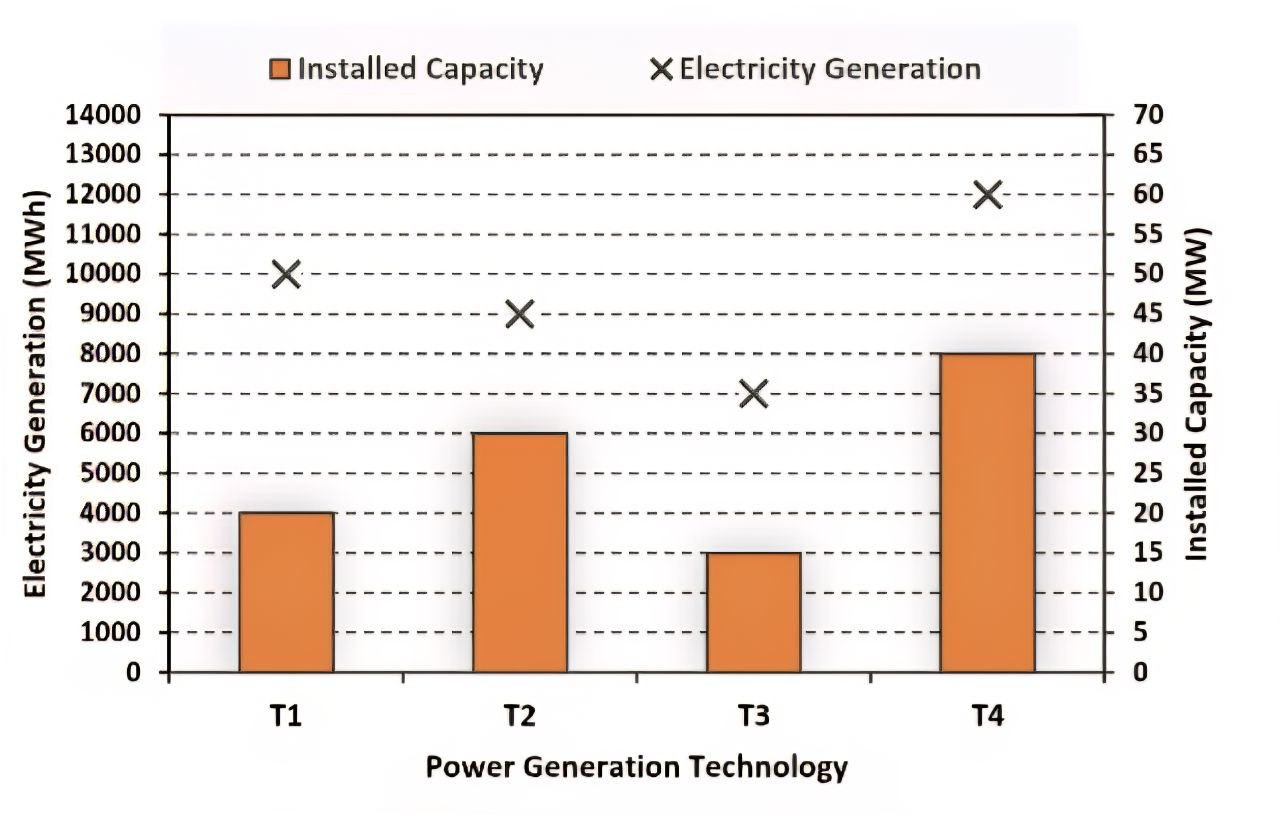
\includegraphics[scale=0.25]{figs/Q8.jpg}
\caption{Power Generation Technology}
\label{Q8}
\end{figure}
\textbf{The Capacity Factor of a power generation technology is:}
$
\text{Capacity Factor} = \frac{\text{Electricity Generation  $\brak{MWh}$}}{\text{Installed Capacity  $\brak{MW}$} \times 1000 \text{  $\brak{h}$}}
$
 Which one of the given technologies has the highest Capacity Factor? 
\hfill $\brak{GATE\ EE\ 2025}$
\begin{enumerate}
\begin{multicols}{4}
\item T1 
  \item T2
  \item T3
 \item T4 \end{multicols}
    \end{enumerate}
   \item In the $4 \times 4$ array shown below, each cell of the first three columns has either a cross  $\brak{X}$ or a number, as per the given rule. 
\textbf{Rule:} The number in a cell represents the count of crosses around its immediate neighboring cells $\brak{left, right, top, bottom, diagonals}$.
As per this rule, the \textbf{maximum} number of crosses possible in the empty column is:
\begin{table}[H]
\centering
\begin{tabular}[12pt]{|c|c|c|c|}
    \hline
    1& 1& 2& \\ 
    \hline
    2& X & 3 & \\
    \hline 
    2 & X & 4 & \\
    \hline
    1 & 2 & X& \\
    \hline   
    \end{tabular} 
\end{table}
\hfill $\brak{GATE\ EE\ 2025}$
    \begin{enumerate}
    \begin{multicols}{4}
\item $0$     
  \item $1$ 
  \item $2$ 
 \item $3$  \end{multicols}
    \end{enumerate}
   \item During a half-moon phase, the Earth-Moon-Sun form a right triangle. If the Moon-Earth-Sun angle at this half-moon phase is measured to be $89.85^\circ$, the ratio of the Earth-Sun and Earth-Moon distances is closest to:     
\hfill $\brak{GATE\ EE\ 2025}$
    \begin{enumerate}
    \begin{multicols}{4}
\item $328$  
  \item $382$   
 \item $238$   
  \item $283$  \end{multicols}
    \end{enumerate}
 \item Amma's tone in the context of the given passage is that of: 
  For Amma, the difference between men and women was a kind of discrimination and inequality; she felt strongly about women's rights but was not familiar with concepts like gender and patriarchy. She would have dismissed Betty Friedan because she was predominantly dealing with the problems of white middle-class women in the United States. Amma, and women of her generation, could de-link the oppression of women from the wider struggle for the liberation of human beings from class exploitation and imperialism. So Amma continued to play her role as mother and wife, but would often complain: 'I am a doormat on which everyone wipes their emotional dirt off'.
\hfill $\brak{GATE\ EE\ 2025}$ 
    \begin{enumerate}
    \begin{multicols}{4}
\item Compromise     
  \item Protest  
  \item Contentment  
  \item Resignation  \end{multicols}
    \end{enumerate}
   \item Fill in the blanks by choosing the correct sequence for the following passage: 
 I am wearing for the first time some  $\brak{i}$\rule{2cm}{0.4pt} that I have never been able to wear for long at a time, as they are horribly tight. I usually put them on just before giving a lecture. The painful pressure they exert on my feet goads my oratorical capacities to their utmost. This sharp and overwhelming pain makes me sing like a nightingale or like one of those Neapolitan singers who also wear  $\brak{ii}$\rule{2cm}{0.4pt} that are too tight. The visceral physical longing, the overwhelming torture provoked by my  $\brak{iii}$\rule{2cm}{0.4pt}  forces me to extract from words distilled and sublime truths, generalized by the supreme inquisition of the pain my  $\brak{iv}$\rule{2cm}{0.4pt} suffer.
\hfill $\brak{GATE\ EE\ 2025}$ 
    \begin{enumerate}
    \begin{multicols}{2}
\item  $\brak{i}$ patent-leather belt  $\brak{ii}$ belts  $\brak{iii}$ patent-leather belt  $\brak{iv}$ waist 
\item  $\brak{i}$ patent-leather shoes  $\brak{ii}$ bands  $\brak{iii}$ patent-leather bands  $\brak{iv}$ wrist 
\item  $\brak{i}$ patent-leather shoes  $\brak{ii}$ shoes  $\brak{iii}$ patent-leather shoes  $\brak{iv}$ feet 
\item  $\brak{i}$ patent-leather jacket  $\brak{ii}$ jacket  $\brak{iii}$ patent-leather jacket  $\brak{iv}$ body \end{multicols}
    \end{enumerate}
  \item The appropriate synonym for the word 'ignite' in the following passage will be: 
Spirituality must be integrated with education. Self-realization is the focus. Each one of us must become aware of our higher self. We are links of a great past to a grand future. We should ignite our dormant inner energy and let it guide our lives. The radiance of such minds embarked on constructive endeavor will bring peace, prosperity and bliss to this nation. 
\hfill $\brak{GATE\ EE\ 2025}$  
    \begin{enumerate}
    \begin{multicols}{4}
\item Encourage 
\item Simulate 
\item  Dissipate 
\item Engross  \end{multicols}
    \end{enumerate}
   \item Which of the following sentences is punctuated correctly? 
\hfill $\brak{GATE\ EE\ 2025}$  
    \begin{enumerate}
    \begin{multicols}{2}
\item One day, I'll write a book, 'I said'. Not just a thriller but a real book, about real people. 
\item 'One day I'll write a book', I said, 'not just a thriller, but a real book, about real people.'
\item 'One day I'll write a book', I said. 'Not just a thriller but, a real book, about real people'.
\item'One day I'll write a book', I said, not just a thriller, but a real book, about real people.' \end{multicols}
    \end{enumerate}
   \item Fill in the blanks with the correct combination of tenses for the given sentence: 
  Darwin's work  $\brak{i}$\rule{2cm}{0.4pt} a related effect that  $\brak{ii}$\rule{2cm}{0.4pt} influenced the development of environmental politics - a 'decentering' of the human being.   
 \hfill $\brak{GATE\ EE\ 2025}$
    \begin{enumerate}
    \begin{multicols}{4}
\item  $\brak{i}$ have  $\brak{ii}$ had 
\item  $\brak{i}$ had  $\brak{ii}$ have 
\item  $\brak{i}$ had  $\brak{ii}$ has 
\item  $\brak{i}$ has  $\brak{ii}$ have
   \end{multicols} \end{enumerate}

   \item Which of the following options holds similar relationship as the words, 'Music: Notes'?  
\hfill $\brak{GATE\ EE\ 2025}$
    \begin{enumerate}
    \begin{multicols}{4}
\item Water: Cold drink 
\item Paper: Class Notes 
\item House: Bricks 
\item Graphite: Charcoal 
\end{multicols}    \end{enumerate}

   \item In a particular code, if "RAMAN" is written as 52 and "MAP" is written as 33, then how will you code "CLICK"?      
\hfill $\brak{GATE\ EE\ 2025}$
    \begin{enumerate}
    \begin{multicols}{4}
\item $37$  
\item $43$  
\item $51$  
\item $38$   \end{multicols}
    \end{enumerate}

   \item On the basis of the statements given below, which valid assumption $\brak{s}$ can be made?    
      Statements:
\begin{enumerate}
    \item Life has suffering
    \item Desire is the cause of suffering
    \item The end of desire is the end of suffering
    \item Desire can be reduced by following the noble eightfold path
\end{enumerate}
Assumptions:
\begin{enumerate}
\begin{multicols}{4}
    \item Suffering is because of wants
    \item Life is not always full of suffering
    \item The eightfold path can reduce suffering
    \item Suffering is caused by life
\end{multicols} \end{enumerate}    
\hfill $\brak{GATE\ EE\ 2025}$
    \begin{enumerate}
    \begin{multicols}{4}
 \item Only 1, 3 and 4  
\item Only 1, 2 and 3  
\item Only 1 and 4  
\item Only 2 and 3  
   \end{multicols} \end{enumerate}
  \item If 'KARAMCHAND' is coded as 'ICPCKEFCLF' what should be the code of 'CREATION'?  
\hfill $\brak{GATE\ EE\ 2025}$
    \begin{enumerate}
    \begin{multicols}{4}
\item ATCCRRKMP  
\item ETGCVKQP  
\item APCCRJMP  
\item ETCGKRPM   \end{multicols}
    \end{enumerate}
   \item { Given an input line of numbers and words, a machine rearranges them following a particular rule in each step. Here is an illustration of an input and rearrangement sequence  $\brak{Step 1 to Step 5}$: \newline
Input: 61 wb ob 48 45 29 34 sb pb lb \newline
Step 1: lb wb ob 48 45 29 34 sb pb 61 \newline
Step 2: lb ob wb 45 29 34 sb pb 61 48 \newline
Step 3: lb ob pb wb 29 34 sb 61 48 45 \newline
Step 4: lb ob pb sb wb 29 61 48 45 34 \newline
Step 5: lb ob pb sb wb 61 48 45 34 29 \newline
Step 5 is the last step of the above arrangement. \newline
Based on the rules followed in the above steps, answer the following question: \newline
Input: cb kb eb 58 49 23 38 jb nb gb 69 82 \newline
Which of the following represents the position of 58 in the fourth step?\\ $\brak{Step-5\ is\ the\ last\ step\ of\ the\ arrangement.}$ }     
\hfill $\brak{GATE\ EE\ 2025}$
    \begin{enumerate}
    \begin{multicols}{4}
\item Second from the left  
\item Fourth from the right  
\item Third from the right  
\item Seventh from the left  
  \end{multicols}  \end{enumerate}
   \item In a certain type of code, they play cricket together' is written as mv kb lb iv'; they score maximum points' is written as gb lb mb kv'; cricket score earned points' is written as mb gv kb kv' and points are earned together' is written as kv mv ob gv.' 
What is the code for earned maximum points'?
\hfill $\brak{GATE\ EE\ 2025}$
    \begin{enumerate}
    \begin{multicols}{4}
\item  gv gb kv       
  \item mv kb mb     
 \item lb iv ob    
  \item ob mv iv    
  \end{multicols}  \end{enumerate}
  \item Which of the statement $\brak{s}$ about the passage weaken $\brak{s}$ the argument presented? 
Scientists associate large brains with greater intelligence. However, in the evolutionary context it has also been identified that beyond a point, the size of the brain has not increased and yet after a particular period, in spite of no significant change in brain size humans have made significant progress. Certain researchers propose that this is because, while the overall brain size may not have changed, marked structural changes can be noticed in specific structures that run parallel to increase in human intelligence.    
\hfill $\brak{GATE\ EE\ 2025}$
    \begin{enumerate}
\item Recent studies refute the hypothesis that region-specific brain development is
necessarily associated with rapid human progress     
  \item Neanderthal people's extinction was probably because of their brain size   
  \item Homo Sapiens and its destruction in the future may happen because of its rapid
brain development   
  \item Recent studies show that Neanderthal people, with relatively smaller brains, were
capable of complex language and social activities   
  \end{enumerate}
  \item The narrator's use of I' in the given passage is/are:    
 I have never been any good at the more lurid sort of writing. Psychopathic killers, impotent war-heroes, self-tortured filmstars, and seedy espionage agents must exist in the world, but strangely enough I do not care across them, and I prefer to write about the people and places I have known and the lives of those poets I have crossed. This crossing of paths makes for stories rather than novels, and although I have worked in both mediums, I am happier being a short-story writer than a novelist. 
\hfill $\brak{GATE\ EE\ 2025}$
    \begin{enumerate}
    \begin{multicols}{2}
\item Self-conscious \
\item Apologetic and regretful 
\item Confessional and communicating 
\item Egotistical and vain
  \end{multicols}  \end{enumerate}
  \item Which of the following recommended action $\brak{s}$ seem to be appropriate with the stated problem?  
      Stated problem: Many students at educational institutes do not attend classes in the post-pandemic scenario.  
     \hfill $\brak{GATE\ EE\ 2025}$
    \begin{enumerate}
  \item Disciplinary action against all students should be taken as a warning.   
  \item Counselling sessions should be organized to address the issues such students face.
  \item Surveys should be conducted to identify the reasons for their absence.
  \item Course content should immediately be changed.
   \end{enumerate}
   \item Read the passage and identify the statement $\brak{s}$ which follow $\brak{s}$ from it: 
      The purpose of this work is to inform educators about the brain science related to emotion and learning, and, more important, to offer strategies to apply these understandings to their own teaching. Although many of the approaches I describe will be familiar, integrating the tiers of emotion and the brain may be a new concept. As an educator I had been trained in how to deliver content and organize my lessons, but I had not been taught how to design learning experiences that support emotions for learning.       
     \hfill $\brak{GATE\ EE\ 2025}$
    \begin{enumerate}
    \item  The author wishes, through his work, to inform us about brain science and learning.    
  \item The author, through his work, wishes to offer strategies to apply our learnings to our teaching.    
  \item The author feels that the newness of his approach lies in linking emotion-oriented approach to health.   
  \item The author wants to use emotions as a strategy for learning.   
   \end{enumerate}
   \item If A says that his mother is the daughter of B's mother, then how is B related to A?      
    \hfill $\brak{GATE\ EE\ 2025}$
    \begin{enumerate}
    \begin{multicols}{4}
  \item Uncle      
  \item Aunt   
  \item Father   
  \item Brother
 \end{multicols}   \end{enumerate}
    \item Which one of the following measures in the Keynesian framework is adopted to tame inflation in an economy?  
    \hfill $\brak{GATE\ EE\ 2025}$
    \begin{enumerate}
    \begin{multicols}{2}
        \item Reduction in government spending
        \item Reduction in the bank rate
        \item Reduction in the repo rate
        \item Increase in merchandise exports
  \end{multicols}  \end{enumerate}
    \item If the difference between actual GDP and the trend output varies inversely with the difference between actual unemployment rate and the natural rate of unemployment, then such a relationship is called the       \hfill $\brak{GATE\ EE\ 2025}$
    \begin{enumerate}
    \begin{multicols}{2}
        \item Okun's law
        \item New Keynesian aggregate supply curve
        \item Taylor Rule
        \item New Keynesian Phillips curve
  \end{multicols}  \end{enumerate}
    \item In the sticky-price model of aggregate supply, if none of the firms in the market have flexible prices, then the short-run aggregate supply curve will be
     \hfill $\brak{GATE\ EE\ 2025}$
    \begin{enumerate}
    \begin{multicols}{2}
        \item horizontal
        \item vertical \\
        \item steeper than it would be if some firms had flexible prices
        \item upward sloping to the right
        \end{multicols}
  \end{enumerate}
\item When transfer of income happens from the ``not richer'' individual to the ``not poorer'' individual, then such a transfer is known as
\hfill $\brak{GATE\ EE\ 2025}$
    \begin{enumerate}
    \begin{multicols}{4}
    \item Regressive transfer
    \item Additive transfer
    \item Direct transfer
    \item Indirect transfer
  \end{multicols}  \end{enumerate}
\item In the context of the Harris-Todaro model of rural-urban migration, which one of the following is TRUE?
\hfill $\brak{GATE\ EE\ 2025}$
    \begin{enumerate}
    \item Unemployment in the urban sector emerges because rural-urban migration occurs primarily due to the higher expected wage income in the urban sector
    \item Unemployment in the urban sector emerges because rural workers migrate to the cities and towns due to the expected shortage of unskilled labour in the urban sector
    \item Unemployment in the urban sector emerges because the rural wage rate is institutionally fixed by the local body at a higher level than the urban wage rate
    \item Unemployment in the rural sector emerges because urban workers migrate to the rural sector due to the higher expected wage income in the advanced economies
  \end{enumerate}
\item The Minimum Support Prices in India are notified based on the recommendations of which one among the following Commissions?
\hfill $\brak{GATE\ EE\ 2025}$
    \begin{enumerate}
    \item Commission for Agricultural Costs and Prices
    \item Commission for Farmers' Benefits and Costs
    \item Commission for Agricultural Subsidy Costs and Prices
    \item Commission for Agricultural Subsidy Benefits and Costs
 \end{enumerate}
\item In an economy, the dependency ratio is the ratio of
\hfill $\brak{GATE\ EE\ 2025}$
    \begin{enumerate}
    \item non-working age group population to the working age group population
    \item number of children to adults in the total population
    \item number of unemployed to employed workers in the total labour force
    \item total foreign aids and grants to the total  $\brak{net}$ factor income from abroad
  \end{enumerate}
\item Which one of the following is NOT a source of finance of the Government of India?
\hfill $\brak{GATE\ EE\ 2025}$
    \begin{enumerate}
    \begin{multicols}{4}
    \item Land revenue
    \item Income tax
    \item Corporate tax
    \item Import duty
 \end{multicols}   \end{enumerate}
\item In the Keynesian closed economy \textit{IS-LM} model, where interest rate is plotted along the vertical axis and output is plotted along the horizontal axis, the product market schedule will be
\hfill $\brak{GATE\ EE\ 2025}$
    \begin{enumerate}
    \item relatively steeper if the interest elasticity of investment is low
    \item relatively steeper, the higher the marginal propensity to save
    \item relatively steeper if the interest elasticity of investment is very high
    \item relatively flatter when the interest elasticity of money demand is very high
    \end{enumerate}
\item In the Keynesian system, the speculative demand for money arises because of
\hfill $\brak{GATE\ EE\ 2025}$
    \begin{enumerate}
    \item uncertainty of future interest rates
    \item uncertainty regarding bond prices and associated capital gains
    \item unexpected out-of-pocket expenditure
    \item the gap that emerges between income and sudden eventual expenditure
   \end{enumerate}
\item Which of the following statements is/are TRUE?
\hfill $\brak{GATE\ EE\ 2025}$
    \begin{enumerate}
     \item A firm experiences economies of scale when an increase in its output of a good or service brings a reduction in the average total cost of production
    \item A firm experiences economies of scope when an increase in its range of goods produced brings down the average total cost of production
    \item A firm experiences economies of scale when an increase in the range of products produced brings down the short-run average total cost of production
    \item A firm experiences economies of scope when an increase in its output of a good or service brings a reduction in the marginal cost of production
   \end{enumerate}
    \item Let $x_1, x_2, \cdots, x_n$ be an independently, and identically distributed  $\brak{\textit{iid}}$ random sample drawn from a population that follows the Normal Distribution $N \brak{\mu, \sigma^2}$, where both the mean $\brak{\mu}$ and variance $ \brak{\sigma^2}$ are unknown. Let $\bar{x}$ be the sample mean. The maximum likelihood estimator  $\brak{MLE}$ of the variance $\brak{\hat{\sigma}^2_{MLE}}$ is/are then characterized by
    \hfill $\brak{GATE\ EE\ 2025}$
    \begin{enumerate}
    \item $\hat{\sigma}_{MLE}^2 = \frac{1}{n}\sum_{i=1}^{n} \brak{x_i-\bar{x}}^2$ which is a biased estimator of $\sigma^2$
    \item $\hat{\sigma}_{MLE}^2 = \frac{1}{n}\sum_{i=1}^{n} \brak{x_i^2-\bar{x}^2}$ which is a consistent estimator of $\sigma^2$
    \item $\hat{\sigma}_{MLE}^2 = \frac{1}{n-1}\sum_{i=1}^{n} \brak{x_i-\bar{x}}^2$ which is an unbiased estimator of $\sigma^2$
    \item $\hat{\sigma}_{MLE}^2 = \frac{1}{n-1}\sum_{i=1}^{n-1} \brak{x_i-\bar{x}}^2$ which is an unbiased and consistent estimator of $\sigma^2$
  \end{enumerate}
\item Consider a simple pooled regression model: $y_{it} = \beta_0 + \beta_1 x_{it} + v_{it}$ where $v_{it} = \mu_i + \epsilon_{it}$ and $Cov \brak{x_{it},\mu_{i}} \neq 0$. Here, $\mu_{i}$ captures the unknown individual specific effects and $\epsilon_{it}$ is the idiosyncratic error uncorrelated with both $x_{it}$ and $\mu_{i}$. If the parameters of this model are estimated using the ordinary least squares  $\brak{OLS}$ method, then the estimated slope coefficient will be
\hfill $\brak{GATE\ EE\ 2025}$
    \begin{enumerate}
    \begin{multicols}{2}
    \item biased
    \item inconsistent
    \item unbiased but consistent
    \item unbiased but efficient
  \end{multicols}  \end{enumerate}
\item Which of the following factor $\brak{s}$ do NOT affect output and employment in the classical macroeconomic model?
\hfill $\brak{GATE\ EE\ 2025}$
    \begin{enumerate}
    \begin{multicols}{2}
    \item Quantity of money
    \item Level of government spending
    \item Level of demand for investment goods
    \item Technological progress
  \end{multicols}  \end{enumerate}
\item For the following function $f \brak{x}$ to be a \textit{probability density function}, the value of $c$ will be \underline{\hspace{2cm}}.  $\brak{\textit{rounded off to two decimal places}}$.
\hfill $\brak{GATE\ EE\ 2025}$  
\begin{align} 
f \brak{x} =
  \begin{cases}
    \frac{c}{\sqrt{x}}, & 0 < x < 4\text{ and } c > 0 \\
    0, & \text{otherwise}
  \end{cases}
 \end{align}
\item A six-face fair die is rolled once, with $X$ being the number that appeared on the uppermost surface. Then the variance of $X$ is \underline{\hspace{2cm}}.  $\brak{\textit{rounded off to three decimal places}}$.
 \hfill $\brak{GATE\ EE\ 2025}$
\item Consider a Cobb-Douglas utility function given as $U \brak{H} =  \brak{24-H}^{1-\alpha} \brak{wH}^\alpha$, where $H$ is the number of hours spent working per day, and $w$ is the wage rate per hour. If $\alpha = \frac{1}{2}$, then the corresponding labour supply  $\brak{in hours} is \underline{\hspace{2cm}}  \brak{\textit{in integer}}$.
 \hfill $\brak{GATE\ EE\ 2025}$
\item For a given foreign currency, if the forward exchange rate of delivery is 20 and the current value of spot exchange rate is 18, then the forward premium will be \underline{\hspace{2cm}}.  $\brak{\textit{rounded off to two decimal places}}$.
 \hfill $\brak{GATE\ EE\ 2025}$
\item Two friends Aditi and Raju are deciding independently whether to watch a movie or go to a music concert that evening. Both friends would prefer to spend the evening together than apart. Aditi would prefer that they watch a movie together, while Raju would prefer that they go to the concert together. The payoff matrix arising from their actions is presented below. $p$ and $ \brak{1-p}$ are the probabilities that Aditi will decide in favour of the movie and concert, respectively. Similarly, $q$ and $ \brak{1-q}$ are the probabilities that Raju will decide in favour of the movie and concert, respectively. Which one of the following options correctly contains all the Nash Equilibria?
\begin{table}[H]
\centering
\begin{tabular}[12pt]{ |c| c| c|} 
    \hline
    & Movie & Concert \\ 
    \hline
    Movie & 2,1 & 0,0  \\
    \hline 
    Concert & 0,0 & 1,2  \\
    \hline
    \end{tabular}
\end{table}
\hfill $\brak{GATE\ EE\ 2025}$
\begin{enumerate}
\begin{multicols}{4}
    \item $ \brak{p=0,\, q=0};$\, $ \brak{p=1,\, q=1};$\, $\brak{ p=\frac{2}{3},\, q=\frac{1}{3} }$
    \item $ \brak{p=0,\, q=1};$\, $ \brak{p=1,\, q=0};$\,  $\brak{ p=\frac{2}{3},\, q=\frac{1}{3} }$
    \item $ \brak{p=0,\, q=0};$\, $ \brak{p=1,\, q=1};$\,  $\brak{ p=\frac{1}{3},\, q=\frac{2}{3}} $
    \item $ \brak{p=0,\, q=1};$\, $ \brak{p=1,\, q=0};$\,  $\brak{ p=\frac{1}{3},\, q=\frac{2}{3} }$ \end{multicols}
\end{enumerate}
\item Consider a two good economy where $a$ denotes consumption of apricots and $b$ denotes consumption of bananas. Anu's utility function is $U^{Anu} \brak{a, b} = a + 2b$, and Binu's utility function is $U^{Binu} \brak{a, b} = \min \brak{a, 2b}$. Anu initially has no apricots and 12 bananas. Binu initially has 12 apricots and no bananas. In the competitive equilibrium, which one of the following will be Anu's optimal consumption bundle?
\hfill $\brak{GATE\ EE\ 2025}$
\begin{enumerate}
\begin{multicols}{4}
    \item 6 apricots and 9 bananas
    \item 9 apricots and 9 bananas
    \item 4 apricots and 10 bananas
    \item 0 apricots and 12 bananas
    \end{multicols}
\end{enumerate}
\item A dual economy consisting of a manufacturing sector  $\brak{M}$ and an agricultural sector  $\brak{A}$ is depicted in the figure below. $O_M O_A$ is the total labour available in the economy of which $O_M L_{SM}$ is the labour supply in the manufacturing sector before any migration was allowed among the labourers. The vertical axis in the left  $\brak{right}$ side measures the wage in the manufacturing, $W_M$  $\brak{agricultural, W_A}$ sector. $LD_M$  $\brak{LD_A}$ is the demand of labour in the manufacturing  $\brak{agricultural}$ sector with respect to $O_M$  $\brak{O_A}$ as the origin. If wages are flexible, and labour is allowed to migrate between these two sectors, then it will be TRUE that
\begin{figure}[H]
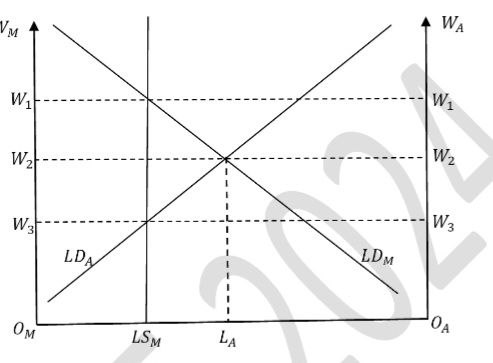
\includegraphics[scale=0.5]{figs/Q47.jpg}
\vspace{0.2cm}
\caption{Graph}
\end{figure}
\hfill $\brak{GATE\ EE\ 2025}$
\begin{enumerate}
   \item Total amount of labour that will migrate from the agricultural sector to the manufacturing sector will be $L_A L_{SM}$
    \item Total amount of labour that will migrate from the manufacturing sector to the agricultural sector will be $L_{SM} L_A$
    \item The wage in the manufacturing sector will be $W_3$
    \item The wage in the agricultural sector will be $W_1$
\end{enumerate}
\item If $X$ and $Y$ are two random variables with the joint probability density function 
\begin{align}
f \brak{x, y} =
\begin{cases}
\frac{2}{3} \brak{x + 2y}; & 0 < x, y < 1 \\
0; & \text{otherwise}
\end{cases}
\end{align}
then $E\sbrak{X|Y=\frac{1}{2}}$ will be
\hfill $\brak{GATE\ EE\ 2025}$
\begin{enumerate}
\begin{multicols}{4}
    \item $\frac{5}{9}$
    \item $\frac{4}{9}$
    \item $\frac{1}{3}$
    \item $\frac{2}{3}$
    \end{multicols}
\end{enumerate}
\item If a discrete random variable $X$ follows the uniform distribution and assumes only the values $8, 9, 11, 15, 18$, and $20$, then $P \brak{|X - 14| < 5}$ is
\hfill $\brak{GATE\ EE\ 2025}$
\begin{enumerate}
\begin{multicols}{4}
    \item $\dfrac{1}{2}$
    \item $\dfrac{1}{5}$
    \item $\dfrac{1}{4}$
    \item $\dfrac{2}{3}$
    \end{multicols}
\end{enumerate}
\item Assume the following probabilities for two events, $A$ and $B$: $P \brak{A} = 0.50$, $P \brak{B} = 0.70$, and $P \brak{A \cup B} = 0.85$. Then we can conclude that
\hfill $\brak{GATE\ EE\ 2025}$
\begin{enumerate}
\begin{multicols}{4}
    \item $A$ and $B$ are mutually independent
    \item $A$ and $B$ are equally likely
    \item $A$ and $B$ are not mutually independent
    \item $A$ and $B$ are mutually exclusive
    \end{multicols}
\end{enumerate}
\item The following table provides different statistical model specifications along with the elasticity of $y_t$ with respect to $x_t$. Which one of the following options is correct?
\begin{table}[H]
\centering
\begin{tabular}{|c|c|c|}
\hline
Row & Statistical Model & Elasticity \\
\hline
1 & $y_t = \beta_1 + \beta_2 \dfrac{1}{x_t} + \epsilon_t$ & $-\dfrac{\beta_2}{x_t^2}$ \\
2 & $y_t = \beta_1 - \beta_2 \ln \brak{x_t} + \epsilon_t$ & $\dfrac{\beta_2}{x_t}$ \\
3 & $\ln \brak{y_t} = \beta_1 + \beta_2 \ln \brak{x_t} + \epsilon_t $ & $\beta_2$ \\
4 & $\ln \brak{y_t} = \beta_1 + \beta_2 x_t + \epsilon_t$ & $\beta_2 x_t$ \\
5 & $\ln \brak{y_t} = \beta_1 + \beta_2 \ln \brak{x_t} + \epsilon_t $ & $\beta_2 \exp \brak{x_t}$ \\
6 & $\ln \brak{y_t} = \beta_1 + \beta_2 x_t + \epsilon_t$ & $\dfrac{\beta_2}{\exp \brak{x_t}}$ \\
\hline
\end{tabular}
\end{table}
\hfill $\brak{GATE\ EE\ 2025}$
\begin{enumerate}
\begin{multicols}{2}
\item Only rows 3 and 4 are correct
\item Only rows 1 and 2 are correct
\item Only rows 3 and 5 are correct
\item Only rows 4 and 6 are correct
\end{multicols}
\end{enumerate}
\item An incumbent firm $\brak{I}$ faces the possibility of entry by a challenger firm $\brak{C}$. If $C$ enters, $I$ may either accommodate or fight. If $C$ does not enter, its payoff is 1, while $I$'s payoff is 2. If $C$ enters, and $I$ accommodates, their payoffs are 2 and 1, respectively. However, if $C$'s entry is met with a fight by $I$, their payoffs are 0 and 1, respectively. Which one of the following is a \textit{subgame perfect Nash equilibrium} $\brak{SPNE}$ under perfect information?
\hfill $\brak{GATE\ EE\ 2025}$
\begin{enumerate}
\begin{multicols}{2}
\item enter; accommodate
\item enter; fight
\item not enter; accommodate
\item not enter; fight
\end{multicols}
\end{enumerate}
\item For the function $F: \mathbb{R}^2 \to \mathbb{R}$ specified as $F\brak{x, y} = x^3 - y^3 + 9xy$, which of the following options is/are correct?
\hfill $\brak{GATE\ EE\ 2025}$
\begin{enumerate}
\begin{multicols}{2}
\item one saddle point
\item one strict local minimum
\item one strict local maximum
\item one global maximum
\end{multicols}
\end{enumerate}
\item A decrease in the income tax rate has a \underline{\hspace{1cm}} effect on the labour supply if the \underline{\hspace{1cm}} effect dominates.
\hfill $\brak{GATE\ EE\ 2025}$
\begin{enumerate}
\begin{multicols}{4}
\item negative; income
\item positive; substitution
\item positive; income
\item negative; substitution
\end{multicols}
\end{enumerate}
\item Which of the following statements is/are FALSE?
\hfill $\brak{GATE\ EE\ 2025}$
\begin{enumerate}
\item The arbitrage pricing theory says that the prices which producers in different countries set for a particular product will be the same if the prices are expressed in the same currency using the current exchange rate
\item The interest rate parity theory says that the interest rates on similar assets in two countries will always be the same
\item The Purchasing Power Parity theory says that the total prices of any basket of products which may split in two different countries will be the same, if the prices are expressed in the same currency using the current exchange rate
\item The real exchange rate between two countries is the rate at which a particular basket of products produced in one country can be traded with a similar basket produced in another country
\end{enumerate}
\item Consider the Solow growth model in which output $\brak{Y}$ is determined by the production function $Y_t = 0.2 K_t^{0.8} + 0.8 L_t$, where $K_t$ and $L_t$ denote capital and labour used in the production process, and $t$ depicts time. The depreciation is given by $\delta K_t$, where $\delta = 0.2$. Saving is given by $sY_t$, where $s$ is the saving rate. If the population does not grow with time, the steady state capital per unit of labour is \underline{\hspace{2cm}} $\brak{in\ integer}$. 
\hfill $\brak{GATE\ EE\ 2025}$
\item Suppose XYZ Corp. is totally financed by equity, it is earning Rs. 2.50 per share; the current market price of the share is Rs. 20.00. There are 10,000 shares outstanding, and the replacement cost of the firm's real assets is Rs. 1,25,000. XYZ Corp.'s value of Tobin's $q$ is \underline{\hspace{2cm}} $\brak{in\ integer}$. 
 \hfill $\brak{GATE\ EE\ 2025}$
\item An industry comprising only two firms produces a homogeneous product where the market demand function is given by $p = 200 - 2\brak{q_1 + q_2}$ where $q_1$ and $q_2$ are the output levels of firm 1 and firm 2, respectively. The individual firm's cost functions are $TC_1 = 4q_1$ and $TC_2 = 4q_2$, where $TC_1$ and $TC_2$ are total costs of firm 1 and 2, respectively. If firm 2 is a Stackelberg Leader, and firm 1 is a follower, then the profit of the Stackelberg Leader will be \underline{\hspace{2cm}} $\brak{rounded\ off\ to\ two\ decimal\ places}$. 
 \hfill $\brak{GATE\ EE\ 2025}$
\item Let $x$ and $y$ be two dummy variables that take the values of either 0 or 1, and follow the bivariate frequency distribution as given below. If a logit regression is estimated with $y$ as the dependent variable and $x$ as the independent variable, then the estimated coefficient of $x$ is \underline{\hspace{2cm}} $\brak{rounded\ off\ to\ two\ decimal\ places}$.
\begin{table}[H]
\centering
\begin{tabular}{|c|c|c|c|}
\hline
 & 0 & 1 & Total \\
\hline
0 & 6 & 11 & 17 \\
1 & 6 & 7 & 13 \\
\hline
Total & 12 & 18 & 30 \\
\hline
\end{tabular}
\end{table}
 \hfill $\brak{GATE\ EE\ 2025}$
\item Based on the table given below, the current account deficit in nominal terms as a percentage of GDP during 2012-13 will be \underline{\hspace{2cm}} $\brak{rounded\ off\ to\ three\ decimal\ places}$.\\
\begin{table}[H]
\centering
\begin{tabular}{|l|c|c|c|}
\hline
Expenditure on Gross Domestic Product $\brak{Rupees in Crores}$ & 2010-11 & 2011-12 & 2012-13 \\
\hline
\textbf{At Current Prices} & & & \\
1. Final Consumption Expenditures & 4865 & 5857 & 6626 \\
2. Gross Fixed Capital Formation & 1388 & 1669 & 1813 \\
3. Changes in Stocks & 65 & 75 & 87 \\
4. Exports of Goods \& Services & 1326 & 1698 & 1674 \\
5. Imports of Goods \& Services & 1786 & 2317 & 2300 \\
\hline
\textbf{At Constant 2004-05 Prices} & & & \\
1. Final Consumption Expenditures & 4039 & 4340 & 4377 \\
2. Gross Fixed Capital Formation & 1026 & 1101 & 1035 \\
3. Changes in Stocks & 52 & 52 & 58 \\
4. Exports of Goods \& Services & 1044 & 1239 & 1193 \\
5. Imports of Goods \& Services & 1348 & 1594 & 1544 \\

\hline
\end{tabular}
\end{table}
 \hfill $\brak{GATE\ EE\ 2025}$
\item In an economy, the effort level of a worker in firm $i$ is denoted by $e_i$ and depends on the wage $W_i$ received by the worker from the firm, and the minimum wage $W_0$ is set by the government. The effort function is given by 
$
e_i\brak{W_i, W_0} = \sqrt{W_i - W_0}
$
If the firm employs $N_i$ unit of workers, then the efficiency unit of labour employed by the firm is $e_i N_i$. The production is based on only the efficiency unit of labour, and the production function is given by
$
F\brak{e_i N_i} = \log_e \brak{e_i N_i}
$
If the minimum wage set by the government is 10, and the profit maximizing firms sell the good in a competitive market at price $P$ by choosing $W_i$ and $N_i$, then the profit maximizing wage set by the firm will be \underline{\hspace{2cm}} $\brak{rounded\ off\ to\ one\ decimal\ place}$. 
 \hfill $\brak{GATE\ EE\ 2025}$
\item In a perfectly competitive market, suppose the market demand curve is given by 
$
P = 10 + W - Q,
$
where $P$ is the market price, $W$ is the average wealth of the consumers in the market, and $Q$ is the industry output. The total cost function for a representative firm is given by $C\brak{q} = q^3 - 2q^2 + 5q$, where $q$ is the output of a firm. If $W = 80$, then the total number of firms in this industry in the long-run will be \underline{\hspace{2cm}} $\brak{in\ integer}$.
 \hfill $\brak{GATE\ EE\ 2025}$
\item The estimated results of a Probit model is given in the table below, where $Y$ is a binary variable taking the value either 0 or 1, and $X$ is an integer. The probability that $Y = 1$ when $X = 30$ is \underline{\hspace{2cm}} $\brak{rounded\ off \ to \ two\ decimal\ places}$.  
\begin{table}[H]
\centering
\begin{tabular}{|c|c|c|c|c|}
\hline
Variable & Coefficient & Standard Error & Z-Statistic & Probability \\
\hline
Constant & -0.064 & 0.399 & -0.161 & 0.871 \\
$X$ & 0.029 & 0.010 & 2.916 & 0.003 \\
\hline
\end{tabular}
\end{table}
 \hfill $\brak{GATE\ EE\ 2025}$
\item Consider an industry with six firms. An analyst collated the data for this industry as given below. The Herfindahl-Hirschman Index $\brak{HHI}$ for this industry will be \underline{\hspace{2cm}} $\brak{in\ integer}$.
\begin{table}[H]
\centering
%64
\begin{tabular}{|c|c|c|}
\hline
 & $b_{1}$ & $b_{2}$ \\
\hline
$a_{1}$ & $(-1,\,3)$ & $(4,\,-1)$ \\
\hline
$a_{2}$ & $(3,\,-4)$ & $(-2,\,2)$ \\
\hline
\end{tabular}

\end{table} 
 \hfill $\brak{GATE\ EE\ 2025}$
\item Consider a duopoly market where Firm 1 and Firm 2 produce differentiated products such that the demand function of each firm is given by:
\begin{align*}
q_1\brak{p_1, p_2} &= 18 - p_1 + p_2  
q_2\brak{p_1, p_2} &= 18 + p_1 - p_2
\end{align*}
Here, $q_1$ and $q_2$ are the outputs produced by Firm 1 and Firm 2, respectively, and $p_1$ and $p_2$ are the corresponding per unit prices. Cost of production for the $i$th firm is given by $C_i\brak{q_i} = 2q_i \quad \forall~i=1,2$. The firms compete in prices. The price set by Firm 2 such that the market is in Nash equilibrium will be \underline{\hspace{2cm}} $\brak{in\ integer}$. 
 \hfill $\brak{GATE\ EE\ 2025}$
\end{enumerate}
\renewcommand{\thefigure}{\theenumi}
\renewcommand{\thetable}{\theenumi}
\end{document}